\section{Modifier les travaux}Ici, vous pouvez voir les t\^aches du poste client, qui ont d\'ej\`a \'et\'e ex\'ecut\'ees et celles qui attendent leur ex\'ecution et les changer en cas \'echeant. Les possibilit\'es de changement suivantes sont \`a votre disposition:\\
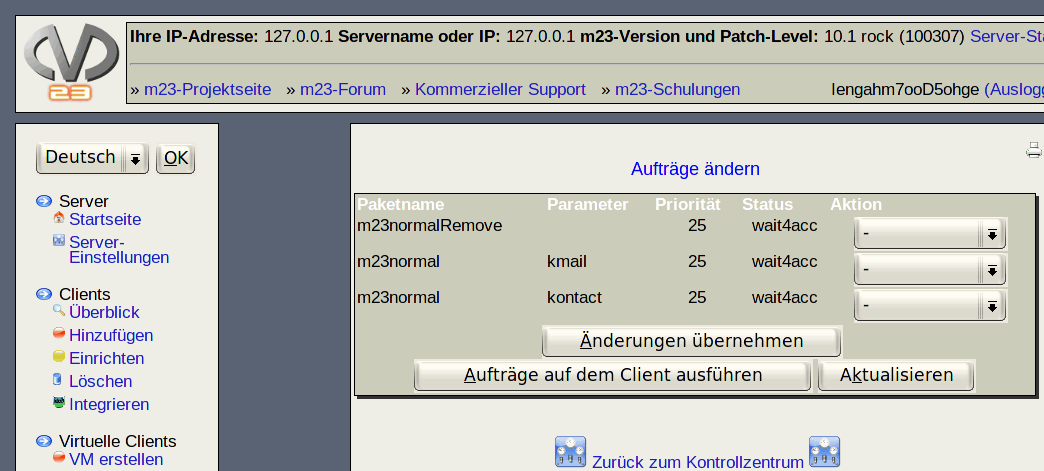
\includegraphics[scale=0.4]{/mdk/doc/manual/screenshots/fr/client_changejobs.png} \\
\begin{itemize}
	\item S\'electionnez \textbf{Effacer} chez \textit{$\ll$Action$\gg$} afin de rejeter la t\^ache d\'efinitivement.\\
	\item \textbf{R�p�ter} d\'eplace une t\^ache d\'ej\`a ex\'ecut\'ee dans la liste des t\^aches \`a accomplir.\\
	\item \textbf{Termin�} marque une t\^ache comme termin\'ee. Celle-ci ne sera plus ex\'ecut\'ee.\\
\end{itemize}
Ensuite, cliquez sur \textit{$\ll$Accepter les changements$\gg$} pour l'enregistrement de vos changements. Si vous voudriez que les t\^aches marqu\'ees avec $\ll$\textbf{R�p�ter}$\gg$ soient ex\'ecut\'ees instantan\'ement, cliquez sur \textit{$\ll$Ex�cuter les travaux sur le poste client$\gg$}.\\
